\chapter{Deployment}

\section{Deployment strategies}

\subsection{Infrastructure deployment}
\begin{itemize}
  \item On premise: Software system installed and run on servers physically located in the
        organization
  \item Hosted: Software system installed on third parties centers
  \item Cloud: Software system is virtualized over the cloud
\end{itemize}


\subsection{Application deployment strategies}

\textbf{Goal}: define how an application, or new versions of it, are deployed
on an infrastructure

\textbf{Main strategies}: In place upgrade, Blue-Green, Canary / Rolling

\subsubsection{In place upgrade}

Installation on top of current version. It requires downtime. All existing settings are preserved


\subsubsection{Blue-green}



\begin{flushleft}
  \begin{minipage}{0.75\linewidth}
    \raggedright
    Two environments, a load balancer directs traffic. Blue env.: where the current application runs. Green: idle

    When a new version is ready for deployment:

    \begin{itemize}
      \item Update deployment, test and monitoring on the green environment
      \item When situation is deemed stable, all traffic is sent to the green env.
      \item The green environment now is the main one, the blue is idle

    \end{itemize}
  \end{minipage}%
  \hfill
  \begin{minipage}{0.2\linewidth}
    \centering

    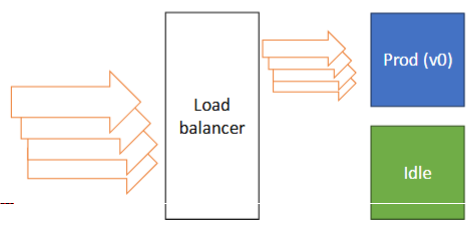
\includegraphics[width=\linewidth]{content/chapters/images/2026-05-23-13-09-03.png}

  \end{minipage}
\end{flushleft}

\subsection{Canary}

\begin{flushleft}
  \begin{minipage}{0.75\linewidth}
    \raggedright

    "Canary in the coal mine".

    Initially, only a few nodes hosts the new deployed application version.
    Load balancer forwards a minority fraction of requests to new version.
    Performances are monitored.
    If there are no severe issues:

    \begin{itemize}
      \item load balancer increases the percentage towards new application version;
      \item The new application is deployed in further nodes
    \end{itemize}

    This incremental process continues until the new version is handling
    all traffic on the majority of nodes, and few ones remains idle, so that
    process can restart with further new versions.

    In case of problems, balance can be temporary reversed
  \end{minipage}%
  \hfill
  \begin{minipage}{0.2\linewidth}
    \centering
    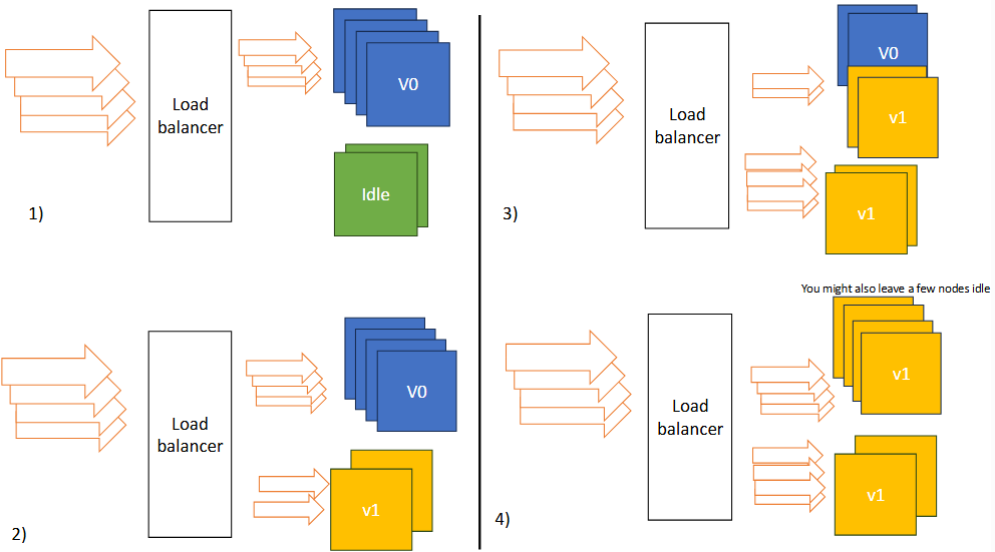
\includegraphics[width=\linewidth]{content/chapters/images/2026-05-23-13-11-36.png}
  \end{minipage}
\end{flushleft}

\begin{flushleft}
  \begin{minipage}[t]{0.45\linewidth}
    \raggedright
    \paragraph{Canary with feature flags}

    \begin{itemize}
      \item New features are flagged in the code, so that they can be enabled
            via configuration files
      \item New features will be enabled for a small groups of users
      \item Monitor the performances of the ``canary'' group
      \item If no significant issues arise, increase dimension of ``canary''
            group
      \item Progressively all users will use the new features
      \item In case of problems, dimensions of canary group can be temporary diminished
    \end{itemize}

  \end{minipage}%
  \hfill
  \begin{minipage}[t]{0.45\linewidth}
    \raggedright

    \paragraph{Rolling with feature flags}

    \begin{itemize}
      \item Same as canary, but exposure of new changes is made on nodes, not
            users
      \item New features are flagged in the code, so that they can be enabled via
            configuration files
      \item New features will be enabled for a small groups of (users) nodes
      \item Monitor the performances of the ``canary'' group
      \item If no significant issues arise, increase dimension of ``canary'' group
      \item Progressively all (users) nodes will use the new features
      \item In case of problems, dimensions of canary group can be temporary diminished
    \end{itemize}


  \end{minipage}
\end{flushleft}


\section{Deployment visualization}

\begin{flushleft}
  \begin{minipage}{0.75\linewidth}
    \raggedright
    \subsubsection{Deployment diagram}

    \textbf{Goal}: describe the mapping of software systems and containers (and
    any other deployable unit) onto deployment nodes

    \textbf{Method}: C4 model with further boundaries for each deployment
    node


    Deployment node: a device or execution environment
    \begin{itemize}
      \item Physical infrastructure (e.g. a physical server or device)
      \item Virtualised infrastructure (e.g. a virtual machine, IaaS)
      \item Containerised infrastructure (e.g. a Docker container)
      \item An execution environment (e.g. a database server)
    \end{itemize}
  \end{minipage}%
  \hfill
  \begin{minipage}{0.2\linewidth}
    \centering
    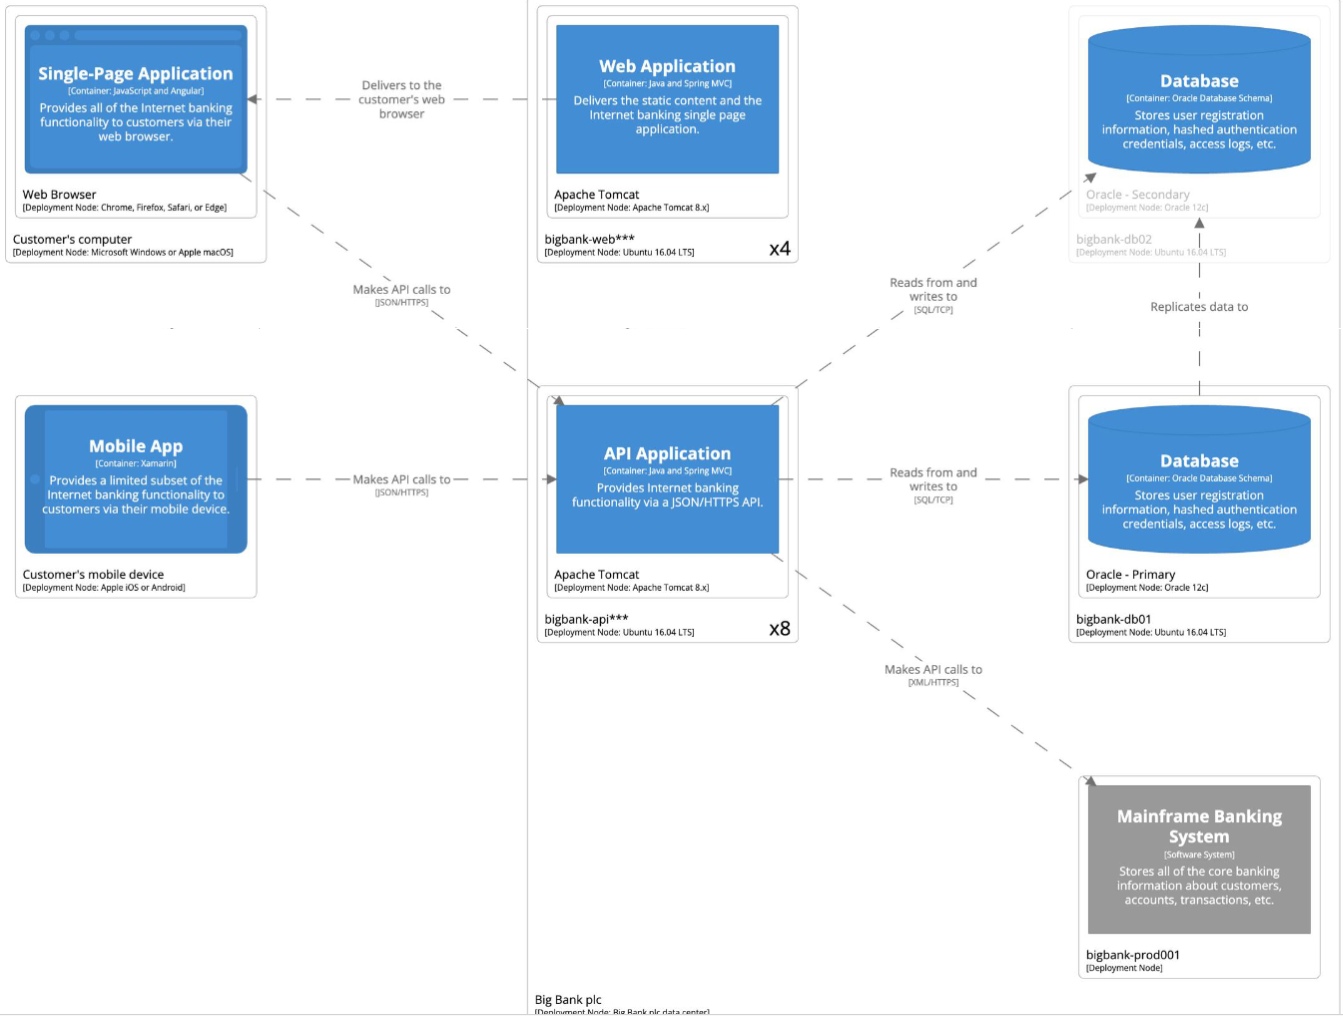
\includegraphics[width=\linewidth]{content/chapters/images/2026-05-23-13-20-11.png}
    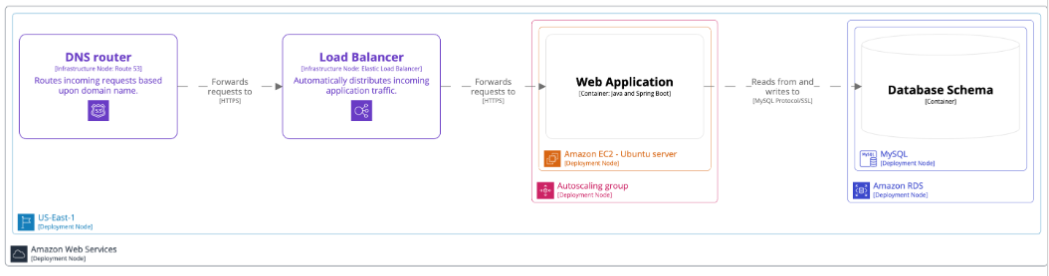
\includegraphics[width=\linewidth]{content/chapters/images/2026-05-23-13-20-30.png}
  \end{minipage}
\end{flushleft}

